
\documentclass[aps,prl,twocolumn,superscriptaddress]{revtex4}

\usepackage{amssymb}
\usepackage{graphicx}
\usepackage{amsmath}

\usepackage{tikz}



\begin{document}
\title{On Periodic Driven Fermi-Hubbard Model}
\author{Ning Sun}
\date{\today}

\begin{abstract}
	We've been studying the problem of periodic driven Fermi-Hubbard model for a while. In this manuscript I write down the model, the method, the analysis and some numerical results of this problem. 
\end{abstract}

\maketitle





\begin{center}
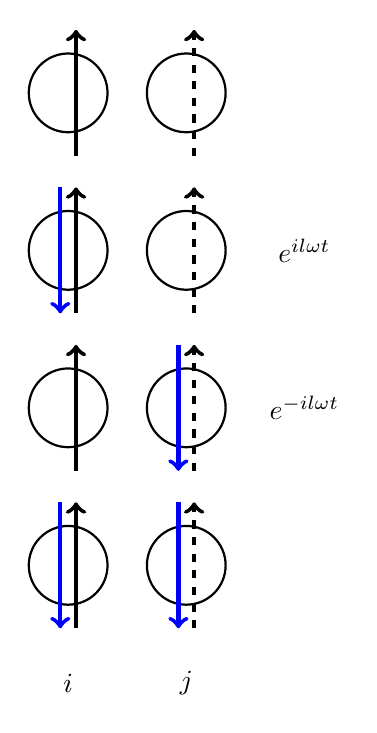
\begin{tikzpicture}
	\draw [thick] (3, 6.5) circle [radius=0.5]; 
	\draw [thick] (4.5, 6.5) circle [radius=0.5]; 
	\draw [->, ultra thick] (3.1, 6.0-.3) -- (3.1, 6.0+1.3);
	\draw [->, dashed, ultra thick] (4.6, 6.0-.3) -- (4.6, 6.0+1.3);

	\draw [thick] (3, 4.5) circle [radius=0.5]; 
	\draw [thick] (4.5, 4.5) circle [radius=0.5];
	\draw [->, ultra thick] (3.1, 4.0-.3) -- (3.1, 4.0+1.3); 
	\draw [->, dashed, ultra thick] (4.6, 4.0-.3) -- (4.6, 4.0+1.3); 
	\draw [<-, blue, ultra thick] (2.9, 4.0-.3) -- (2.9, 4.0+1.3);
	\node at (6, 4.5) {$e^{i l\omega t}$}; 

	\draw [thick] (3, 2.5) circle [radius=0.5]; 
	\draw [thick] (4.5, 2.5) circle [radius=0.5];
	\draw [->, ultra thick] (3.1, 2.0-.3) -- (3.1, 2.0+1.3);
	\draw [->, dashed, ultra thick] (4.6, 2.0-.3) -- (4.6, 2.0+1.3); 
	\draw [<-, blue, ultra thick] (4.4, 2.0-.3) -- (4.4, 2.0+1.3);
	\node at (6, 2.5) {$e^{-i l\omega t}$}; 

	\draw [thick] (3, 0.5) circle [radius=0.5]; 
	\draw [thick] (4.5, 0.5) circle [radius=0.5]; 
	\draw [->, ultra thick] (3.1, -.3) -- (3.1, 1.3);
	\draw [->, dashed, ultra thick] (4.6, -.3) -- (4.6, 1.3);
	\draw [<-, blue, ultra thick] (2.9, -.3) -- (2.9, 1.3);
	\draw [<-, blue, ultra thick] (4.4, -.3) -- (4.4, 1.3);

	\node at (3, -1.) {$i$}; 
	\node at (4.5, -1.) {$j$}; 

\end{tikzpicture}
\end{center}



\begin{center}
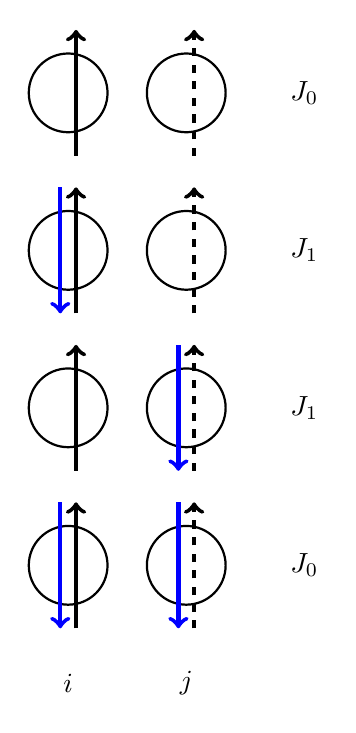
\begin{tikzpicture}
	\draw [thick] (3, 6.5) circle [radius=0.5]; 
	\draw [thick] (4.5, 6.5) circle [radius=0.5]; 
	\draw [->, ultra thick] (3.1, 6.0-.3) -- (3.1, 6.0+1.3);
	\draw [->, dashed, ultra thick] (4.6, 6.0-.3) -- (4.6, 6.0+1.3);
	\node at (6, 6.5) {$J_0$};

	\draw [thick] (3, 4.5) circle [radius=0.5]; 
	\draw [thick] (4.5, 4.5) circle [radius=0.5];
	\draw [->, ultra thick] (3.1, 4.0-.3) -- (3.1, 4.0+1.3); 
	\draw [->, dashed, ultra thick] (4.6, 4.0-.3) -- (4.6, 4.0+1.3); 
	\draw [<-, blue, ultra thick] (2.9, 4.0-.3) -- (2.9, 4.0+1.3);
	\node at (6, 4.5) {$J_1$}; 

	\draw [thick] (3, 2.5) circle [radius=0.5]; 
	\draw [thick] (4.5, 2.5) circle [radius=0.5];
	\draw [->, ultra thick] (3.1, 2.0-.3) -- (3.1, 2.0+1.3);
	\draw [->, dashed, ultra thick] (4.6, 2.0-.3) -- (4.6, 2.0+1.3); 
	\draw [<-, blue, ultra thick] (4.4, 2.0-.3) -- (4.4, 2.0+1.3);
	\node at (6, 2.5) {$J_1$}; 

	\draw [thick] (3, 0.5) circle [radius=0.5]; 
	\draw [thick] (4.5, 0.5) circle [radius=0.5]; 
	\draw [->, ultra thick] (3.1, -.3) -- (3.1, 1.3);
	\draw [->, dashed, ultra thick] (4.6, -.3) -- (4.6, 1.3);
	\draw [<-, blue, ultra thick] (2.9, -.3) -- (2.9, 1.3);
	\draw [<-, blue, ultra thick] (4.4, -.3) -- (4.4, 1.3);
	\node at (6, 0.5) {$J_0$};

	\node at (3, -1.) {$i$}; 
	\node at (4.5, -1.) {$j$}; 

\end{tikzpicture}
\end{center}



\begin{center}
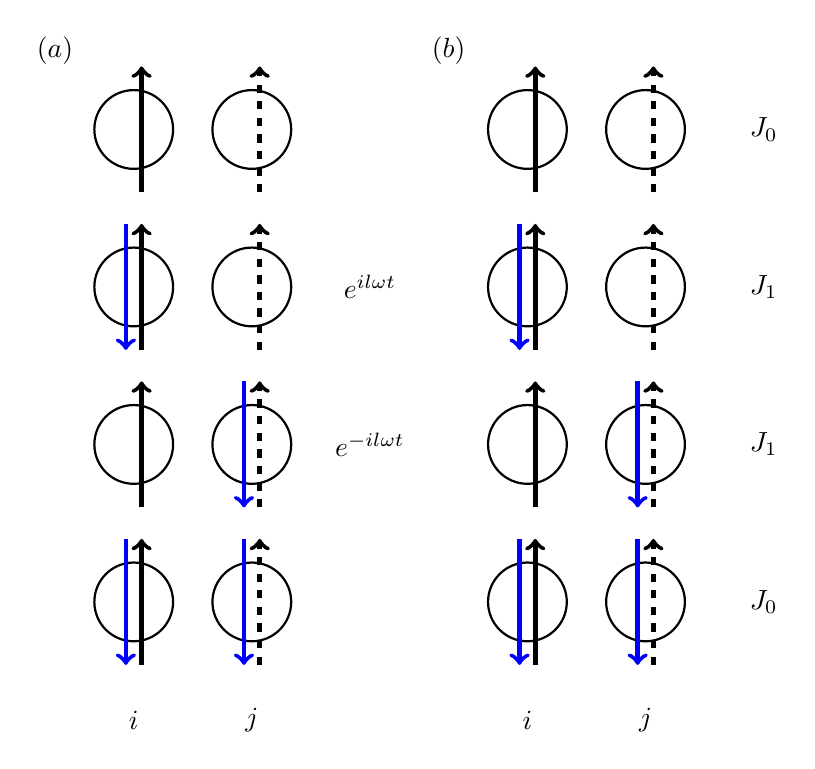
\begin{tikzpicture}

	\draw [thick] (3, 6.5) circle [radius=0.5]; 
	\draw [thick] (4.5, 6.5) circle [radius=0.5]; 
	\draw [->, ultra thick] (3.1, 6.0-.3) -- (3.1, 6.0+1.3);
	\draw [->, dashed, ultra thick] (4.6, 6.0-.3) -- (4.6, 6.0+1.3);
	% \node at (6, 6.5) {$J_0$};

	\draw [thick] (3, 4.5) circle [radius=0.5]; 
	\draw [thick] (4.5, 4.5) circle [radius=0.5];
	\draw [->, ultra thick] (3.1, 4.0-.3) -- (3.1, 4.0+1.3); 
	\draw [->, dashed, ultra thick] (4.6, 4.0-.3) -- (4.6, 4.0+1.3); 
	\draw [<-, blue, ultra thick] (2.9, 4.0-.3) -- (2.9, 4.0+1.3);
	\node at (6, 4.5) {$e^{i l\omega t}$}; 

	\draw [thick] (3, 2.5) circle [radius=0.5]; 
	\draw [thick] (4.5, 2.5) circle [radius=0.5];
	\draw [->, ultra thick] (3.1, 2.0-.3) -- (3.1, 2.0+1.3);
	\draw [->, dashed, ultra thick] (4.6, 2.0-.3) -- (4.6, 2.0+1.3); 
	\draw [<-, blue, ultra thick] (4.4, 2.0-.3) -- (4.4, 2.0+1.3);
	\node at (6, 2.5) {$e^{-i l\omega t}$}; 

	\draw [thick] (3, 0.5) circle [radius=0.5]; 
	\draw [thick] (4.5, 0.5) circle [radius=0.5]; 
	\draw [->, ultra thick] (3.1, -.3) -- (3.1, 1.3);
	\draw [->, dashed, ultra thick] (4.6, -.3) -- (4.6, 1.3);
	\draw [<-, blue, ultra thick] (2.9, -.3) -- (2.9, 1.3);
	\draw [<-, blue, ultra thick] (4.4, -.3) -- (4.4, 1.3);
	% \node at (6, 0.5) {$J_0$};

	\node at (3, -1.) {$i$}; 
	\node at (4.5, -1.) {$j$}; 
	\node at (2, 7.5) {$(a)$}; 

	%%%%%%%%%%%%%%%%%%%%%%%%%%%%%%%%%%%%%%%%%%%%%%%%%%%%%%%%%%%%%%%%

	\draw [thick] (3+5, 6.5) circle [radius=0.5]; 
	\draw [thick] (4.5+5, 6.5) circle [radius=0.5]; 
	\draw [->, ultra thick] (3.1+5, 6.0-.3) -- (3.1+5, 6.0+1.3);
	\draw [->, dashed, ultra thick] (4.6+5, 6.0-.3) -- (4.6+5, 6.0+1.3);
	\node at (6+5, 6.5) {$J_0$};

	\draw [thick] (3+5, 4.5) circle [radius=0.5]; 
	\draw [thick] (4.5+5, 4.5) circle [radius=0.5];
	\draw [->, ultra thick] (3.1+5, 4.0-.3) -- (3.1+5, 4.0+1.3); 
	\draw [->, dashed, ultra thick] (4.6+5, 4.0-.3) -- (4.6+5, 4.0+1.3); 
	\draw [<-, blue, ultra thick] (2.9+5, 4.0-.3) -- (2.9+5, 4.0+1.3);
	\node at (6+5, 4.5) {$J_1$}; 

	\draw [thick] (3+5, 2.5) circle [radius=0.5]; 
	\draw [thick] (4.5+5, 2.5) circle [radius=0.5];
	\draw [->, ultra thick] (3.1+5, 2.0-.3) -- (3.1+5, 2.0+1.3);
	\draw [->, dashed, ultra thick] (4.6+5, 2.0-.3) -- (4.6+5, 2.0+1.3); 
	\draw [<-, blue, ultra thick] (4.4+5, 2.0-.3) -- (4.4+5, 2.0+1.3);
	\node at (6+5, 2.5) {$J_1$}; 

	\draw [thick] (3+5, 0.5) circle [radius=0.5]; 
	\draw [thick] (4.5+5, 0.5) circle [radius=0.5]; 
	\draw [->, ultra thick] (3.1+5, -.3) -- (3.1+5, 1.3);
	\draw [->, dashed, ultra thick] (4.6+5, -.3) -- (4.6+5, 1.3);
	\draw [<-, blue, ultra thick] (2.9+5, -.3) -- (2.9+5, 1.3);
	\draw [<-, blue, ultra thick] (4.4+5, -.3) -- (4.4+5, 1.3);
	\node at (6+5, 0.5) {$J_0$};

	\node at (3+5, -1.) {$i$}; 
	\node at (4.5+5, -1.) {$j$}; 
	\node at (2+5, 7.5) {$(b)$}; 

\end{tikzpicture}
\end{center}










\end{document}